\documentclass[border=5pt,tikz]{standalone}
\usepackage{tkz-graph}
\begin{document}

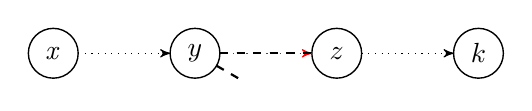
\begin{tikzpicture}[scale=0.9]
  \tikzset{
    vertex/.style = {circle,fill=black!100,minimum size=20pt,inner sep=0pt},
    edge/.style = {->,> = latex'},
  }
  \def\vr{6mm}
  \def\nb{6}
  \Vertex[L=\textit{x},x=-2,y=0]{x}
  \Vertex[L=$y$,x=0,y=0]{y}
  \Vertex[L=$z$,x=2,y=0]{z}
  \Vertex[L=$k$,x=4,y=0]{k}
  
  \draw[dotted][->,>=stealth'] (x)--(y);
  \draw[dotted][->,>=stealth',red](y)--(z);
  \draw[dotted][->,>=stealth'](z)--(k);
  
  \draw[dashed,thick] (y)--(z);
  \draw[dashed,thick] (y) -- (z);

  \tikzset{
    VertexStyle/.append style={label=$t_{y}$},
  }
  \draw[dashed,thick](y) -- ++ (-30:.8cm);

\end{tikzpicture}
\end{document}